\chapter{Arquitectura del sistema y compilación}

El desarrollo de una aplicación gráfica interactiva como \textit{Copper}
requiere una base estructural robusta que garantice la separación de
responsabilidades, la mantenibilidad y la escalabilidad del código. Una
arquitectura de software bien definida es fundamental para gestionar la
complejidad inherente a la renderización en tiempo real, la gestión del estado
de la escena y la interacción con el usuario.

En este capítulo se presenta un análisis detallado de la arquitectura de
\textit{Copper}. El sistema no sigue de forma estricta ningún patrón de diseño,
sino que implementa una arquitectura por componentes con una fuerte
inspiración en el patrón Modelo-Vista-Controlador (MVC). Este enfoque
pragmático permite que cada componente se especialice en una tarea concreta
(renderizado, lógica de la escena, control de entrada), interactuando con otros
para construir la funcionalidad completa de la aplicación.

A continuación, se describirán los componentes principales, sus
responsabilidades y las interacciones entre ellos.

\section{Visión General de la Arquitectura}

La arquitectura de \textit{Copper} se puede descomponer en cuatro capas lógicas
principales que encapsulan las diferentes funcionalidades, como se ve en la
Figura\ref{fig:diagrama_arquitectura}.

\begin{figure}[H]
    \begin{center}
    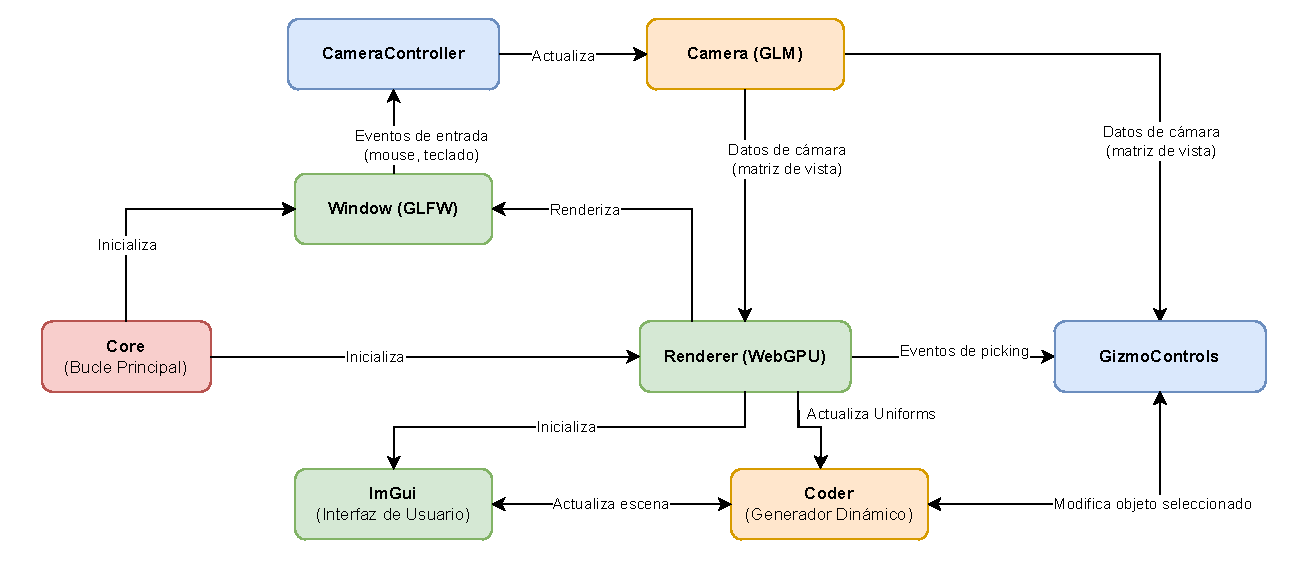
\includegraphics[width=0.95\textwidth]{imagenes/diagrama_arquitectura.pdf}
    \end{center}
    \caption{Diagrama de la arquitectura por componentes de \textit{Copper}.}
    \label{fig:diagrama_arquitectura}
\end{figure}

Las capas identificadas son:

\begin{itemize}
    \item \textbf{Capa de Orquestación y Ciclo de Vida (rojo):} Responsable de inicializar, ejecutar y terminar la aplicación. Es el punto de entrada y el gestor del bucle principal.
    \item \textbf{Capa de Datos y Lógica de la Escena (Modelo) (naranja):} Contiene el estado de la escena 3D, incluyendo los objetos, sus propiedades y la cámara. Encapsula la lógica de negocio, como la generación dinámica de shaders.
    \item \textbf{Capa de Presentación (Vista) (verde):} Se encarga de toda la representación visual, tanto el renderizado de la escena 3D mediante WebGPU como la interfaz gráfica de usuario (GUI) construida con ImGui.
    \item \textbf{Capa de Control de Usuario (Controlador) (azul):} Captura y procesa las entradas del usuario (ratón y teclado) y las traduce en acciones que modifican el estado del Modelo o la Vista.
\end{itemize}

Esta separación permite que, por ejemplo, se pueda modificar el motor de
renderizado (\texttt{Renderer}) sin afectar a la lógica de la escena
(\texttt{Coder}), o cambiar la forma en que se controla la cámara
(\texttt{CameraController}) sin alterar su representación de datos
(\texttt{Camera}).

\section{Análisis de Componentes por Capa}

A continuación, se detallan los componentes clave dentro de cada capa lógica,
referenciando sus ficheros de implementación.

\subsection{Capa de Orquestación y Ciclo de Vida}

El núcleo de la aplicación reside en la clase \texttt{Core}, definida en
\texttt{src/core/Core.h} y \texttt{src/core/Core.cpp}.

\begin{description}
    \item[\texttt{Core}:] Actúa como el orquestador principal. Su responsabilidad es inicializar todos los subsistemas en el orden correcto (\texttt{Core::Initialize}), gestionar el bucle principal de la aplicación (\texttt{Core::MainLoop}) y liberar los recursos de forma ordenada al finalizar (\texttt{Core::Terminate}). El bucle principal consulta el estado de la ventana y delega la tarea de dibujado al \texttt{Renderer} en cada fotograma.
\end{description}

\subsection{Capa de Datos y Lógica de la Escena (Modelo)}

Esta capa representa el estado y la lógica de negocio de la aplicación.

\begin{description}
    \item[\texttt{Coder} (\texttt{src/core/Coder.h}, \texttt{.cpp})]: Es el componente central del modelo. Gestiona la lista de objetos 3D de la escena (\texttt{std::vector<Object>}), sus propiedades (posición, color, forma) y las operaciones booleanas entre ellos. Su responsabilidad más crítica es el método \texttt{generateShaderCode()}, que traduce dinámicamente el estado de los objetos en código de shader WGSL. Este mecanismo es la "lógica de negocio" principal de \textit{Copper}, ya que define cómo se representa visualmente la escena. También se encarga de la persistencia de la escena mediante las funciones \texttt{saveScene()} y \texttt{loadScene()}.

    \item[\texttt{Camera} (\texttt{src/core/Camera.h}, \texttt{.cpp})]: Representa los datos y el estado de la cámara virtual. Almacena la matriz de vista (\texttt{view\_matrix}) y proporciona métodos para acceder a sus vectores fundamentales (posición, dirección, etc.). Aunque es una entidad pasiva, es una parte fundamental del modelo de datos, ya que define la perspectiva desde la que se observa la escena.
\end{description}

\subsection{Capa de Presentación (Vista)}

Esta capa es responsable de todo lo que el usuario ve en la pantalla.

\begin{description}
    \item[\texttt{Renderer} (\texttt{src/core/Renderer.h}, \texttt{.cpp})]: Es la vista principal. Su función es dibujar la escena 3D utilizando la API WebGPU. Orquesta el proceso de renderizado en su método \texttt{Render()}, donde toma los datos del \texttt{Coder} y la \texttt{Camera}, actualiza los \textit{uniforms} del shader y ejecuta los comandos de dibujado. También gestiona recursos de la GPU como la \textit{pipeline} de renderizado y los búferes.

    \item[\texttt{Interfaz} (\texttt{src/ui/Interfaz.h}, \texttt{.cpp})]: Componente especializado de la vista que gestiona la Interfaz Gráfica de Usuario (GUI) mediante la biblioteca ImGui. Es responsable de crear todos los paneles, botones y controles deslizantes que permiten al usuario interactuar con la aplicación. Lee el estado directamente del \texttt{Coder} para mostrar las propiedades de los objetos y, a su vez, invoca métodos en el \texttt{Coder} para modificar dicho estado, lo que representa una desviación del patrón MVC estricto.

    \item[\texttt{Window} (\texttt{src/ui/Window.h}, \texttt{.cpp})]: Gestiona la ventana nativa de la aplicación utilizando GLFW. Proporciona el "lienzo" sobre el que dibujan el \texttt{Renderer} y la \texttt{Interfaz}. Además, es responsable de registrar y despachar los eventos de entrada del sistema operativo (como clics de ratón o cambios de tamaño) a los componentes correspondientes.
\end{description}

\subsection{Capa de Control de Usuario (Controlador)}

Esta capa gestiona la entrada del usuario y la traduce en comandos para el
Modelo y la Vista.
\begin{description}
    \item[\texttt{CameraController} (\texttt{src/core/CameraController.h}, \texttt{.cpp})]: Es un controlador especializado en la manipulación de la cámara. Captura los eventos de arrastre del ratón y la rueda de desplazamiento para calcular la nueva orientación y posición de la cámara. En su método \texttt{update\_camera()}, modifica directamente el estado del objeto \texttt{Camera} (el Modelo) para reflejar la interacción del usuario.

    \item[\texttt{GizmoControls} (\texttt{src/core/GizmoControls.h}, \texttt{.cpp})]: Otro controlador altamente especializado, dedicado a la manipulación de los gizmos de transformación de los objetos. Cuando el usuario interactúa con un gizmo, esta clase calcula el desplazamiento correspondiente y actualiza la posición del objeto seleccionado. El nuevo estado se comunica al \texttt{Coder} para que la escena se actualice.

    \item[\texttt{Renderer} como despachador de eventos]: Excepcionalmente, la clase \texttt{Renderer} también asume un rol de controlador, debido al picking realizado por shader. Su método \texttt{OnMouseButton()} actúa como un punto de entrada que decide si la acción del usuario corresponde a una selección de objeto (lo que desencadena la pipeline de \textit{picking}) o a la manipulación de un gizmo (delegando el control a \texttt{GizmoControls}).
\end{description}

\section{Conclusiones sobre la Arquitectura}

La arquitectura de \textit{Copper} puede definirse como un sistema basado en
componentes con una clara separación de responsabilidades, que se alinea con
los principios del patrón Modelo-Vista-Controlador (MVC) sin seguir su
implementación más estricta.

La separación es evidente:
\begin{itemize}
    \item \textbf{Modelo}: \texttt{Coder} y \texttt{Camera} contienen el estado y la lógica central.
    \item \textbf{Vista}: \texttt{Renderer} e \texttt{Interfaz} se ocupan de la presentación visual.
    \item \textbf{Controlador}: \texttt{CameraController} y \texttt{GizmoControls} gestionan la entrada del usuario de forma aislada.
\end{itemize}

Sin embargo, se observan desviaciones pragmáticas del patrón MVC clásico, como
la comunicación directa entre la Vista (\texttt{Interfaz}) y el Modelo
(\texttt{Coder}) para modificar propiedades de objetos. Este enfoque, común en
aplicaciones gráficas, reduce la complejidad al eliminar la necesidad de un
controlador intermediario para cada pequeña modificación de estado.

En conclusión, la estructura elegida es eficaz y adecuada para una aplicación
de modelado 3D. Promueve la cohesión dentro de cada componente y mantiene un
bajo acoplamiento entre las distintas capas lógicas, lo que facilita el
mantenimiento, la depuración y la futura expansión del software.

\section{Sistema de construcción y compilación del proyecto}

El proyecto utiliza \textbf{CMake} como sistema de construcción para gestionar
la compilación, las dependencias y la organización de los archivos fuente.
CMake es una herramienta ampliamente empleada en proyectos de desarrollo de
software en C y C++ por su capacidad para generar archivos de construcción para
distintos sistemas y entornos \cite{cmake-docs}.

\subsection{Estructura del archivo CMake}

En la raíz del proyecto se encuentra el archivo \texttt{CMakeLists.txt}, que
define la configuración de la construcción. Sus principales componentes y
funcionalidades son:

\begin{itemize}
    \item \textbf{Definición del proyecto:}\\
          El proyecto se denomina \texttt{Copper}, está configurado para compilar en C++20 y se identifica como una aplicación de modelado 3D basada en SDF:
          \begin{lstlisting}[language=CMake, caption={Definición del proyecto en CMakeLists.txt}]
            project(Copper VERSION 0.0.2 LANGUAGES CXX C DESCRIPTION "3D SDF-based modeling application")
            set(CMAKE_CXX_STANDARD 20)
            set(CMAKE_CXX_STANDARD_REQUIRED ON)
            set(CMAKE_CXX_EXTENSIONS OFF)
\end{lstlisting}

    \item \textbf{Gestión de dependencias externas:}\\
          El archivo especifica la inclusión y compilación de bibliotecas externas necesarias para el funcionamiento del proyecto, como Dawn (WebGPU), GLM (matemáticas), ImGuiFileDialog (diálogos de archivos en la interfaz gráfica), y las fuentes de ImGui. La gestión de dependencias se realiza mediante \texttt{add\_subdirectory} y \texttt{FetchContent}, permitiendo su descarga y compilación automática junto al proyecto principal.
          Es importante el uso de \texttt{DAWN\_FETCH\_DEPENDENCIES} para no tener que instalar todas las librerías que usa Dawn ya que estos son pesados y pueden no ser necesarios, y así evitamos gestionar manualmente las dependencias.

    \item \textbf{Organización de los archivos fuente:}\\
          Se recopilan y organizan los archivos fuente del proyecto, excluyendo explícitamente el fichero \texttt{main.cpp} para evitar duplicidad, y se añaden los archivos fuente de ImGui.
          \begin{lstlisting}[language=CMake, caption={Organización de los archivos fuente en CMakeLists.txt}]
            file(GLOB_RECURSE COPPER_SOURCES src/*.cpp src/*.h)
            list(REMOVE_ITEM COPPER_SOURCES ${CMAKE_SOURCE_DIR}/src/main.cpp)\end{lstlisting}

    \item \textbf{Creación del ejecutable:}\\
          Se define el ejecutable principal \texttt{copper}, que se compila a partir de \texttt{main.cpp}, los archivos fuente propios y los de ImGui.
          \begin{lstlisting}[language=CMake, caption={Creación del ejecutable en CMakeLists.txt}]
    add_executable(copper src/main.cpp ${COPPER_SOURCES} ${IMGUI_SOURCES})\end{lstlisting}

    \item \textbf{Definición de directorios de inclusión:}\\
          Se especifican los directorios que contienen los archivos de cabecera para facilitar la compilación.
          \begin{lstlisting}[language=CMake, caption={Definición de directorios de inclusión en CMakeLists.txt}]
    target_include_directories(copper PRIVATE src lib/imgui lib/imgui/misc/cpp lib/imgui/backends ${CMAKE_CURRENT_BINARY_DIR}/src)\end{lstlisting}

    \item \textbf{Vinculación de bibliotecas:}\\
          Se vinculan las bibliotecas necesarias para el funcionamiento del programa, como Dawn/WebGPU, GLM, GLFW y el soporte para WebGPU en GLFW.
          \begin{lstlisting}[language=CMake, caption={Vinculación de bibliotecas en CMakeLists.txt}]
    target_link_libraries(copper PRIVATE dawn::webgpu_dawn glm::glm glfw webgpu_glfw ImGuiFileDialog)\end{lstlisting}

    \item \textbf{Definiciones de compilador:}\\
          Se incluyen definiciones específicas que permiten, por ejemplo, indicar el directorio de recursos y activar la integración de ImGui con WebGPU usando Dawn.
          \begin{lstlisting}[language=CMake, caption={Definiciones de compilador en CMakeLists.txt}]
                target_compile_definitions(copper PRIVATE RESOURCE_DIR="${CMAKE_CURRENT_SOURCE_DIR}/src" IMGUI_IMPL_WEBGPU_BACKEND_DAWN)
\end{lstlisting}
\end{itemize}

\subsection{Proceso de compilación}

El desarrollo principal se ha llevado a cabo sobre un entorno Linux, aunque la
elección de herramientas y librerías multiplataforma debería asegurar su compilación en
otros sistemas operativos como Windows o macOS, esto podría requerir ajustes en
la configuración del proyecto.

Para compilar el proyecto, se debe disponer de CMake y un compilador compatible
con C++20. El proceso estándar usando git para compilar el proyecto consiste
en:

\begin{enumerate}
    \item Si fuese necesario añadir los paquetes utilizados por Dawn:
          \begin{lstlisting}[language=bash]
        sudo apt-get install libxrandr-dev libxinerama-dev libxcursor-dev mesa-common-dev libx11-xcb-dev pkg-config nodejs npm\end{lstlisting}
    \item Clonar el repositorio de Git y actualizar los submódulos:
          \begin{lstlisting}[language=bash]
        git clone https://github.com/tu-usuario/copper.git
        cd copper
        git submodule update --init\end{lstlisting}
    \item Compilar en la carpeta build:
          \begin{lstlisting}[language=bash]
        cmake -B build
        cmake --build build -j$(nproc)\end{lstlisting}
    \item Por último si se quiere ejecutar el proyecto:
          \begin{lstlisting}[language=bash]
        ./build/copper\end{lstlisting}
\end{enumerate}

Esto construirá el ejecutable \texttt{copper}, incluyendo todas las
dependencias y archivos fuente indicados en \texttt{CMakeLists.txt}.

\subsection{Función del sistema de construcción}

El sistema CMake facilita:

\begin{itemize}
    \item La gestión automática de dependencias externas.
    \item La configuración multiplataforma.
    \item La compilación eficiente de todos los módulos del programa, asegurando que las
          dependencias y rutas de inclusión están correctamente resueltas.
    \item La integración de recursos y librerías de terceros necesarios para la ejecución
          (por ejemplo, ImGui para la interfaz gráfica, Dawn para el acceso a WebGPU).
\end{itemize}

La configuración descrita en el archivo \texttt{CMakeLists.txt} permite
reproducir el proceso de compilación en distintos sistemas, facilitando el
trabajo colaborativo y la portabilidad del proyecto.